\newpage
\chapter{METODE PENELITIAN} \label{Bab III}

\section{Alur Penelitian} \label{III.Alur}
Penelitian ini berfokus pada evaluasi skalabilitas, generalisasi lintas-dataset, dan efisiensi komputasi dari keluarga arsitektur MedMamba (MedMamba-T, MedMamba-S, dan MedMamba-B) pada klasifikasi citra penyakit kulit yang tidak seimbang. Alur pelaksanaan penelitian secara terstruktur ditunjukkan pada diagram berikut (\textit{flowchart}) seperti yang terlihat pada Gambar \ref{fig:3.alur}. \par

\begin{figure}[H] 
    \centering
    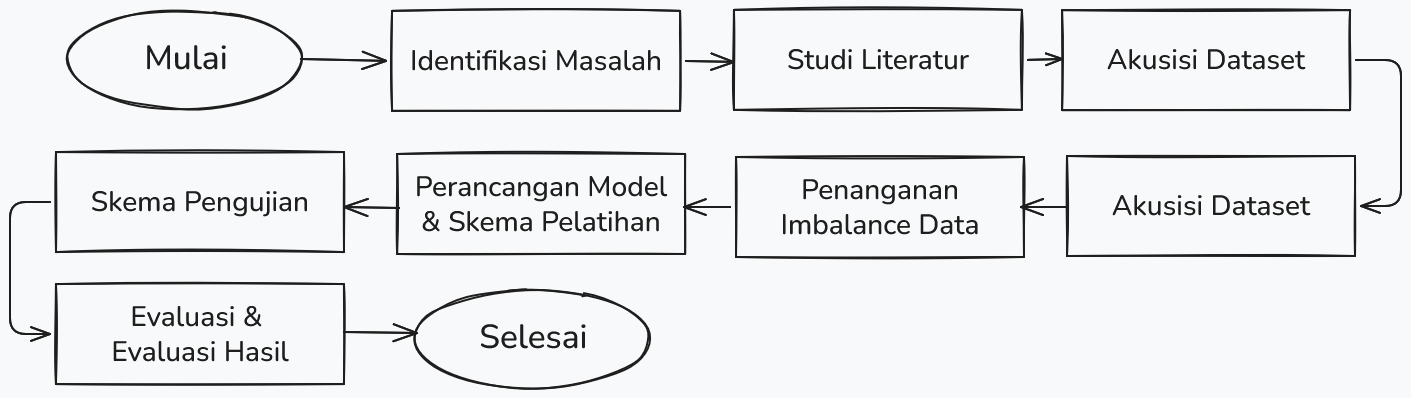
\includegraphics[width=0.9\textwidth]{figure/Diagram Alur.jpeg}
    \caption{Alur Penelitian}
    \label{fig:3.alur}
\end{figure}

\section{Penjabaran Langkah Penelitian} \label{III.Jabar Alur}
Penjelasan dari setiap langkah pada alur penelitian akan dijelaskan secara merinci untuk memberikan detail yang jelas terhadap metode yang digunakan. Berikut penjelasan dari setiap langkah penelitian tersebut. \par

\subsection{Identifikasi Masalah} \label{III.Identifikasi}
Tahap awal yang dilakukan sebelum memulai penelitian adalah identifikasi masalah. Identifikasi dilakukan dengan cara menelaah secara mendalam karakteristik dataset dermatologi medis serta keterbatasan arsitektur model klasifikasi yang ada saat ini. Pada klasifikasi penyakit kulit menggunakan dataset DermaMNIST, ditemukan adanya ketidakseimbangan kelas yang sangat ekstrem di mana kelas mayoritas \textit{Melanocytic Nevi} (\texttt{nv}) mendominasi hingga $\sim$67\% dari keseluruhan sampel, sedangkan kelas minoritas seperti \textit{Dermatofibroma} (\texttt{df}) dan \textit{Vascular Lesions} (\texttt{vasc}) masing-masing hanya mencakup $\sim$1,14\% dan $\sim$1,41\% data. Kondisi ketimpangan ini memicu bias prediksi pada fungsi kerugian konvensional dan menurunkan sensitivitas model terhadap penyakit langka \cite{hariz2026analisis}. Selain itu, investigasi kualitas data mengungkapkan ditemukannya kebocoran data (\textit{data leakage}) sebesar 13,47\% pada DermaMNIST murni akibat pemisahan berbasis gambar (\textit{image-level split}), yang mengakibatkan inflasi performa secara semu \cite{abhishek2025investigating}. Di sisi lain, penggunaan arsitektur \textit{Vision Transformer} (ViT) memicu masalah baru berupa kompleksitas komputasi kuadratik $\mathcal{O}(N^2)$ yang sangat membebani memori VRAM \cite{dosovitskiy2021image}. Berdasarkan permasalahan tersebut, penelitian ini mengevaluasi arsitektur \textit{State Space Models} (MedMamba) ber-kompleksitas linear $\mathcal{O}(N)$ pada dataset terkoreksi (\textit{DermaMNIST-C} dan \textit{Fitzpatrick17k-C}) untuk mengatasi masalah ketidakseimbangan data, kebocoran data, dan keterbatasan efisiensi komputasi pada perangkat \textit{Edge AI}. \par


\subsection{Studi Literatur} \label{III.Studi}
Tahap studi literatur dilakukan dengan mengumpulkan, mempelajari, dan mengkaji berbagai sumber akademis terpercaya yang diterbitkan dalam kurun waktu lima tahun terakhir (2021--2026). Referensi yang dikumpulkan berfokus pada lima pilar utama, yaitu: konsep dasar pemrosesan sekuensial linear berbasis \textit{State Space Models} (SSM) dan modul \textit{Visual State Space} (VSSM) pada arsitektur Mamba \cite{gu2024mamba, yue2024medmamba}, temuan investigasi integritas dataset medis terkait \textit{data leakage} dan duplikasi \cite{abhishek2025investigating}, paradigma \textit{Supervised Contrastive Learning} (SupCon) untuk ekstraksi representasi fitur yang robust \cite{khosla2020supervised}, teknik penanganan \textit{imbalanced data} melalui \textit{Class-Weighted Loss} dan augmentasi hibrida \cite{salmi2024imbalanced, qi2025mediaug}, serta metrik evaluasi keandalan klinis seperti \textit{Expected Calibration Error} (ECE) \cite{guo2017calibration} dan metrik efisiensi \textit{hardware} \cite{lavaei2025resource}. Tahap studi literatur ini bertujuan untuk membangun landasan teoritis yang kokoh serta memberikan kerangka acuan yang valid dalam menyusun skenario eksperimen dan menganalisis hasil pengujian. \par

\subsection{Akuisisi Dataset} \label{III.Akuisisi}
Proses pengumpulan data dalam penelitian ini dilakukan dengan mengunduh dataset publik dari repositori resmi Zenodo dan MedMNIST \cite{yang2023medmnist}. Tiga himpunan data utama yang diakuisisi meliputi \textit{DermaMNIST-C}, \textit{Fitzpatrick17k-C}, dan \textit{DermaMNIST-origin}. Dataset \textit{DermaMNIST-C} terdiri dari 10.015 citra dermatoskopi yang telah dibersihkan dari kebocoran data menggunakan pemisahan terisolasi di tingkat pasien/lesi (\textit{lesion-level disjoint split}) \cite{abhishek2025investigating}. Dataset \textit{Fitzpatrick17k-C} berisi 11.394 citra medis klinis (\textit{in-the-wild}) yang telah dibersihkan dari duplikasi dan kesalahan label, serta dilengkapi dengan anotasi skala warna kulit \textit{Fitzpatrick Skin Tone} (FST I--VI) dan partisi baku \textit{train-validation-test} (70:10:20) \cite{abhishek2025investigating, groh2021evaluating}. Sementara itu, dataset \textit{DermaMNIST-origin} diikutsertakan secara khusus sebagai pembanding untuk mengkuantifikasi secara eksperimental seberapa besar dampak kebocoran data terhadap inflasi skor akurasi model. \par

\subsection{Preprocessing Data} \label{III.Preprocessing}
Tahap \textit{preprocessing data} dilakukan untuk menyiapkan citra medis agar berada dalam format baku yang optimal sebelum dimasukkan ke dalam proses pelatihan model. Langkah pertama adalah penyesuaian resolusi citra (\textit{resizing}) secara langsung dari citra resolusi tinggi/asli menjadi dimensi $224 \times 224$ piksel menggunakan interpolasi \textit{bicubic}. Metode ini dipilih untuk menghindari efek pikselasi buruk dan hilangnya detail morfologi halus pada struktur lesi yang biasa terjadi pada metode \textit{upscaling nearest neighbor} \cite{abhishek2025investigating}. Langkah selanjutnya adalah normalisasi nilai intensitas piksel, di mana rentang nilai piksel $[0, 255]$ dikonversi menjadi tensor berformat \textit{floating-point} (\textit{float}) pada rentang $[0.0, 1.0]$, kemudian distandarisasi menggunakan nilai rata-rata (\textit{mean}) dan deviasi standar (\textit{standard deviation}) terhitung dari populasi dataset. \par

\subsection{Penanganan Imbalanced Data dan Augmentasi} \label{III.Imbalanced}
Guna mengatasi ketimpangan distribusi kelas pada dataset \textit{DermaMNIST-C}, diterapkan kombinasi strategi di tingkat fungsi kerugian dan manipulasi data latih. Pada tingkat algoritma, diterapkan \textit{Class-Weighted Cross-Entropy Loss} ($\mathcal{L}_{CWCE}$) yang secara otomatis menghitung bobot penalti terbalik berdasarkan frekuensi kemunculan sampel pada tiap kelas, sehingga memaksa gradien model untuk memberikan perhatian lebih pada kelas-kelas minoritas \cite{salmi2024imbalanced}. Pada tingkat data, diterapkan teknik \textit{Hybrid Data Augmentation} secara khusus pada porsi data latih kelas minoritas (seperti \texttt{df}, \texttt{vasc}, dan \texttt{akiec}). Teknik augmentasi hibrida ini menggabungkan transformasi geometris mencakup pencerminan acak (\textit{Random Horizontal/Vertical Flip}) dan rotasi acak hingga 20 derajat, dengan transformasi fotometrik berupa manipulasi warna (\textit{Color Jitter}) serta penghapusan daerah piksel acak (\textit{Random Erasing}). Penerapan teknik ini bertujuan untuk memperkaya variasi visual sampel minoritas tanpa mengubah label biologisnya \cite{qi2025mediaug}. \par 

\subsection{Perancangan Model dan Skenario Pelatihan} \label{III.Perancangan}
Tahap perancangan model diawali dengan mengonfigurasi tiga skala arsitektur \textit{Visual State Space Model} (MedMamba) \cite{yue2024medmamba}, yaitu \textit{MedMamba-T} ($\sim$14,5M parameter) sebagai pembanding \textit{lightweight}, \textit{MedMamba-S} ($\sim$22,8M parameter) sebagai fokus utama penelitian, dan \textit{MedMamba-B} ($\sim$47,1M parameter) sebagai \textit{baseline upper-bound}. Pelatihan dilakukan dalam dua paradigma terpisah: \textit{Supervised Learning} terawasi langsung dan \textit{Supervised Contrastive Learning} (SupCon). Pada paradigma SupCon, \textit{backbone} MedMamba dilatih terlebih dahulu pada tahap \textit{pre-training} untuk memetakan proyeksi fitur ke dalam ruang laten menggunakan \textit{contrastive loss}, sebelum dilanjutkan dengan \textit{fine-tuning} pada lapisan klasifikasi linier. Proses pelatihan dieksekusi menggunakan \textit{AdamW optimizer}, \textit{Cosine Annealing Learning Rate Scheduler}, dan optimasi \textit{Automatic Mixed Precision} (AMP) FP16 untuk menghemat memori. Untuk menjamin reproduksibilitas dan kestabilan hasil statistik, penguncian benih acak (\textit{multi-seed}) diterapkan, serta pengujian berbasis \textit{5-Fold Cross Validation} dijalankan pada dataset yang tidak memiliki pemisahan baku. \par

\subsection{Evaluasi Model} \label{III.Evaluasi}
Tahap evaluasi dilakukan untuk mengukur dan menganalisis kinerja model yang telah dilatih berdasarkan tiga dimensi utama \cite{grandini2020metrics}. Dimensi pertama adalah performa diagnostik klinis multikelas yang diukur menggunakan metrik \textit{Balanced Accuracy}, \textit{Macro Precision}, \textit{Macro Recall}, \textit{Macro F1-Score}, serta \textit{Matthews Correlation Coefficient} (MCC) untuk menjamin penilaian yang adil pada kondisi \textit{imbalanced class}. Dimensi kedua adalah reliabilitas kalibrasi prediksi yang diukur melalui \textit{Expected Calibration Error} (ECE) guna menilai sejauh mana tingkat kepercayaan prediksi (\textit{confidence score}) model selaras dengan akurasi aktualnya. Dimensi ketiga adalah efisiensi komputasi fisik yang diukur secara langsung pada GPU laptop NVIDIA RTX 2050 (4 GB VRAM), meliputi konsumsi VRAM puncak (\textit{peak VRAM}), latensi inferensi per sampel (ms), \textit{throughput} (citra/detik), serta jumlah parameter terparameterisasi dan GFLOPs. \par

\section{Alat dan Bahan Tugas Akhir} \label{III.Alat dan Bahan}
Berisi alat-alat dan bahan-bahan yang digunakan dalam penelitian. \par

\subsection{Alat} \label{III.Alat}
Berikut merupakan alat-alat yang digunakan dalam pelaksanaan penelitian: \par
\begin{enumerate}[noitemsep]
	\item \textit{Laptop} yang dilengkapi dengan unit pemroses grafis NVIDIA GeForce RTX 2050 Laptop GPU berkapasitas memori 4 GB GDDR6 VRAM berbasis arsitektur Ampere dengan \textit{Compute Capability} 8.6. Perangkat keras pendukung mencakup pemroses utama \textit{multi-core} dan memori sistem sebesar 16 GB RAM DDR4.
	\item Arch Linux
	\item Github
	\item Python 3.10
	\item CUDA Toolkit 12.1
	\item Code editor Microsoft Visual Studio Code, Google Colab, dan Kaggle Notebook 
	\item Library Python: PyTorch, numpy, pandas, scikit-learn, matplotlib, seaborn.
\end{enumerate}

\subsection{Bahan Penelitian} \label{III.Bahan}
Bahan utama yang digunakan dalam penelitian ini terdiri dari tiga himpunan data citra medis publik serta satu bobot \textit{pretrained}. Bahan pertama adalah dataset \textit{DermaMNIST-C} yang berisi 10.015 citra dermatoskopi terkoreksi dan bebas dari kebocoran data melalui pemisahan terisolasi di tingkat pasien/lesi (\textit{lesion-level disjoint split}) \cite{abhishek2025investigating}. Bahan kedua adalah dataset \textit{Fitzpatrick17k-C} yang mencakup 11.394 citra medis klinis (\textit{in-the-wild}) terkoreksi, bebas dari duplikasi dan kesalahan label, serta dilengkapi dengan anotasi warna kulit \textit{Fitzpatrick Skin Tone} (FST I--VI) \cite{groh2021evaluating}. Bahan ketiga adalah dataset \textit{DermaMNIST-origin} yang diikutsertakan secara khusus untuk menguji dampak langsung kebocoran data. Bahan terakhir adalah bobot \textit{pretrained} \texttt{Medmamba.pth} \cite{yue2024medmamba} yang diuji pemuatannya secara parsial (\textit{partial initialization}) untuk dibandingkan efektivitasnya terhadap pelatihan dari awal (\textit{random initialization}). \par

\section{Metode Pengembangan} \label{III.Metode}
Metode pengembangan sistem berfokus pada perancangan arsitektur model \textit{State Space Models}, penerapan paradigma pelatihan terawasi dan kontrastif, serta strategi mitigasi ketidakseimbangan data medis. \par

\subsection{Arsitektur Model MedMamba} \label{III.ArsitekturMedMamba}
Arsitektur MedMamba menggabungkan lapisan konvolusi untuk ekstraksi fitur lokal spasial dengan modul \textit{Visual State Space} (VSSM). Modul VSSM mengintegrasikan \textit{Cross-Scan Module} (CSM) \cite{liu2024vmamba} yang memindai citra 2D secara linier $\mathcal{O}(N)$ ke empat arah spasial mendatar dan tegak guna memodelkan konteks global tanpa beban memori kuadratik $\mathcal{O}(N^2)$ seperti pada \textit{Vision Transformer} (ViT). Penelitian ini menguji tiga varian skala MedMamba untuk memetakan \textit{trade-off} antara kapasitas parameter dan efisiensi komputasi, meliputi \textit{MedMamba-T} (\textit{Tiny}) dengan kedalaman \texttt{depths = } dan dimensi \texttt{dims = } ($\sim$14,5M parameter) sebagai pembanding \textit{lightweight}, \textit{MedMamba-S} (\textit{Small}) dengan kedalaman \texttt{depths = } dan dimensi \texttt{dims = } ($\sim$22,8M parameter) sebagai fokus utama penelitian, serta \textit{MedMamba-B} (\textit{Base}) dengan kedalaman \texttt{depths = } dan dimensi \texttt{dims = } ($\sim$47,1M parameter) sebagai \textit{baseline upper-bound}. \par

\subsection{Supervised vs. Contrastive Learning} \label{III.ParadigmaPelatihan}
Pelatihan model dikembangkan melalui dua paradigma utama. Paradigma pertama adalah \textit{Supervised Learning} langsung yang melatih model secara \textit{end-to-end} menggunakan \textit{Class-Weighted Cross-Entropy Loss} ($\mathcal{L}_{CWCE}$) dengan pengoptimasi \textit{AdamW}, penjadwal \textit{Cosine Annealing Learning Rate} dengan $T_{max}$ terikat durasi epoch, serta optimasi \textit{Automatic Mixed Precision} (AMP) FP16 untuk menjamin efisiensi alokasi memori VRAM. Paradigma kedua adalah \textit{Supervised Contrastive Learning} (SupCon) \cite{khosla2020supervised} yang dibagi ke dalam dua tahap. Pada tahap pertama, \textit{backbone} MedMamba dilatih menggunakan \textit{SupCon Loss} dengan parameter temperatur $\tau = 0,07$ untuk mendekatkan vektor representasi fitur dari kelas yang sama dan memisahkan kelas yang berbeda di ruang laten. Pada tahap kedua, lapisan klasifikasi linier dipasang di atas \textit{backbone} terfasilitasi tersebut untuk mengeksekusi prediksi label target secara langsung. \par

\subsection{Strategi Mitigasi Data Tak Seimbang} \label{III.StrategiMitigasi}
Strategi penanganan data tak seimbang dikembangkan pada dua tingkatan terpisah. Pada tingkat algoritma, bobot penalti fungsi kerugian dihitung secara otomatis berdasarkan frekuensi terbalik populasi kelas untuk memberikan penalti gradien yang lebih besar pada kesalahan prediksi kelas langka \cite{cui2019classbalanced}. Pada tingkat manipulasi data, diterapkan teknik \textit{Hybrid Data Augmentation} secara khusus pada porsi data latih kelas minoritas seperti \texttt{df}, \texttt{vasc}, dan \texttt{akiec}. Augmentasi hibrida menggabungkan pembalikan acak (\textit{Random Horizontal/Vertical Flip}) dan rotasi acak hingga 20 derajat untuk variasi geometris, serta manipulasi warna (\textit{Color Jitter}) dan penghapusan daerah piksel acak (\textit{Random Erasing}) untuk meningkatkan variasi fotometrik tanpa merusak informasi morfologi lesi \cite{shorten2019survey}. \par

\section{Rancangan Pengujian dan Skema Eksperimen} \label{III.RancanganPengujian}
Rancangan pengujian disusun ke dalam lima skenario eksperimen utama untuk menjawab seluruh hipotesis penelitian secara komprehensif. Skenario pertama adalah \textit{In-Dataset Benchmark} yang mengevaluasi performa dasar ketiga varian MedMamba pada data bersih menggunakan pengujian \textit{5-Fold Cross Validation} pada \textit{DermaMNIST-C} dan pembagian partisi baku 70:10:20 pada \textit{Fitzpatrick17k-C}. Skenario kedua adalah \textit{Leakage Impact Test} yang melatih model pada \textit{DermaMNIST-origin} kemudian mengujinya pada \textit{DermaMNIST-C} dan \textit{Fitzpatrick17k-C} guna mengkuantifikasi secara mendalam seberapa besar persentase akurasi yang terinflasi akibat kebocoran data. \par

Skenario ketiga adalah \textit{Cross-Dataset Generalization} yang menguji daya tahan transferabilitas fitur antar-domain medis secara \textit{zero-shot}, di mana model yang dilatih pada \textit{DermaMNIST-C} diuji secara langsung pada \textit{Fitzpatrick17k-C} (Arah A), dan sebaliknya model yang dilatih pada \textit{Fitzpatrick17k-C} diuji pada \textit{DermaMNIST-C} (Arah B). Skenario keempat adalah \textit{Joint-Dataset Training} yang menggabungkan populasi data latih \textit{DermaMNIST-C} dan \textit{Fitzpatrick17k-C} menjadi satu himpunan heterogen, lalu menguji performanya pada gabungan himpunan uji. Skenario kelima adalah \textit{Studi Ablasi MedMamba-S} yang dieksekusi secara terisolasi pada \textit{DermaMNIST-C} untuk membedah kontribusi spesifik dari penggunaan \textit{Class-Weighted Loss}, inisialisasi bobot (\textit{Random} vs \textit{Partial Pretrained}), serta variasi penjadwalan \textit{learning rate}. \par

\section{Metrik Evaluasi} \label{III.MetrikEvaluasi}
Kinerja dari setiap model yang dievaluasi diukur dan dianalisis secara kualitatif dan kuantitatif berdasarkan tiga dimensi utama. \par

\subsection{Metrik Performa Klasifikasi Multikelas} \label{III.MetrikKlasifikasi}
Berdasarkan nilai \textit{Confusion Matrix} multikelas ($TP_c, FP_c, TN_c, FN_c$), dihitung metrik \textit{Balanced Accuracy} (Macro Recall) untuk mengukur rata-rata sensitivitas seluruh kelas tanpa terdistorsi oleh populasi mayoritas:
\begin{equation}
	\text{Balanced Accuracy} = \frac{1}{C} \sum_{c=1}^{C} \frac{TP_c}{TP_c + FN_c}
\end{equation}
Selain itu, dihitung pula metrik \textit{Macro F1-Score} untuk mengukur keseimbangan antara \textit{Precision} dan \textit{Recall} secara rata-rata tidak terbobot:
\begin{equation}
	\text{Macro F1-Score} = \frac{1}{C} \sum_{c=1}^{C} \frac{2 \cdot \text{Precision}_c \cdot \text{Recall}_c}{\text{Precision}_c + \text{Recall}_c}
\end{equation}
Untuk mengevaluasi keandalan klasifikasi multikelas pada kondisi ketimpangan kelas yang ekstrem secara lebih adil, dihitung metrik \textit{Matthews Correlation Coefficient} (MCC) \cite{chicco2023mcc}:
\begin{equation}
	\text{MCC} = \frac{c \cdot s - \sum_{k}^{C} p_k t_k}{\sqrt{\left(s^2 - \sum_{k}^{C} p_k^2\right) \left(s^2 - \sum_{k}^{C} t_k^2\right)}}
\end{equation}
di mana $c$ adalah total sampel yang terklasifikasi benar, $s$ adalah total sampel, $p_k$ adalah jumlah kali kelas $k$ diprediksi, dan $t_k$ adalah jumlah kali kelas $k$ benar-benar muncul. \par

\subsection{Metrik Reliabilitas Kalibrasi Prediksi} \label{III.MetrikKalibrasi}
Guna menjamin keamanan klinis agar skor kepercayaan prediksi (\textit{confidence score}) selaras dengan akurasi aktualnya, diukur metrik \textit{Expected Calibration Error} (ECE) \cite{guo2017calibration}. Pengukuran dilakukan dengan mengelompokkan $N$ sampel ke dalam $M$ bin interval kepercayaan $B_m$ yang berjarak sama (misalnya $M = 10$):
\begin{equation}
	\text{ECE} = \sum_{m=1}^{M} \frac{|B_m|}{N} \left| \text{acc}(B_m) - \text{conf}(B_m) \right|
\end{equation}
di mana $\text{acc}(B_m)$ menyatakan akurasi aktual dalam bin $B_m$ dan $\text{conf}(B_m)$ menyatakan rata-rata nilai kepercayaan prediksi pada bin tersebut. Sebagai metrik pendukung, dihitung pula nilai \textit{Brier Loss} untuk menilai kesalahan kuadrat rata-rata antara probabilitas prediksi dengan vektor \textit{one-hot} label sebenarnya. \par

\subsection{Metrik Efisiensi Komputasi Hardware} \label{III.MetrikKomputasi}
Efisiensi komputasi fisik diukur secara langsung pada GPU laptop NVIDIA RTX 2050 (4 GB VRAM) mencakup empat indikator utama \cite{aalishah2025medmambalite}. Indikator pertama adalah konsumsi VRAM puncak (\textit{Peak VRAM Allocated}) yang dihitung dalam satuan megabyte/gigabyte menggunakan fungsi pemantauan memori internal PyTorch. Indikator kedua adalah latensi inferensi per sampel (\textit{Inference Latency}) yang diukur dalam milidetik (ms) pada ukuran \textit{batch} sama dengan satu. Indikator ketiga adalah \textit{Throughput} yang mengukur jumlah citra yang berhasil diproses per detik (\textit{images per second}). Indikator keempat adalah jejak fisik model yang dihitung melalui jumlah parameter terparameterisasi (dalam jutaan/M) serta total operasi titik kambang (\textit{Giga Floating Point Operations} / GFLOPs). \par